% Propuesta — primera entrega. Compila: pdflatex propuesta_primera_entrega.tex (2 veces)
\documentclass[conference]{IEEEtran}
\usepackage[spanish]{babel}
\usepackage{cite}
\usepackage{booktabs}
\usepackage{graphicx}
\usepackage[hidelinks]{hyperref}

\begin{document}

\title{Triage de alertas SOC sobre 2M de eventos (Precinct6): propuesta de proyecto}

\author{\IEEEauthorblockN{Author Name}
\IEEEauthorblockA{Curso: Aprendizaje Autom\'atico --- Semestre 8}
}

\maketitle

\begin{abstract}
Los SOC se ahogan en alertas: 2,011,674 eventos en 6 d\'ias con solo 0.38\% malicioso (IR 245:1).
Proponemos construir un sistema de triage que clasifique cada evento en benigno/sospechoso/malicioso
con probabilidades, pistas MITRE ATT\&CK y decisi\'on operativa en $<$50\,ms.
Presentamos la motivaci\'on, dos casos de literatura verificados (Devign, CVSS-BERT),
el dise\~no de la soluci\'on en cascada (tabular $\to$ texto $\to$ grafo) con su diagrama,
y el dataset con visualizaciones exploratorias.
\end{abstract}

\section{Introducci\'on y motivaci\'on}

Un Centro de Operaciones de Seguridad (SOC) vigila la infraestructura con decenas de productos
(syslog, auditor\'ia Windows, flujos VPC, telemetr\'ia endpoint). WitFoo Precinct correlaciona
todo con 261 reglas en \emph{incidentes} (se\~nales + subgrafo de proveniencia + reporte).
El problema a abordar es el \textbf{triage de alertas}: dado un evento, predecir su tier
\texttt{benign} / \texttt{suspicious} / \texttt{malicious} con probabilidades calibradas,
hints ATT\&CK y decisi\'on \texttt{escalar} vs.\ \texttt{monitorear} en $<$50\,ms para rankear la cola.

Es importante por volumen (2M de eventos en 6 d\'ias, imposible a mano), por desbalance extremo
(0.38\% malicioso: el accuracy miente, un siempre-benigno acierta 94\%), por el cambio de contexto
del analista (necesita mensaje + MITRE + cadena, no un n\'umero), porque las etiquetas ser\'an
correlaci\'on autom\'atica imperfecta (Unprocessed en 2,005,877/2,011,674), y porque hay deriva
temporal (malicious termina 07-30, benigno sigue a 08-01: el split deber\'a ser temporal, no shuffle).

\section{Revisi\'on de literatura}

\textbf{Caso 1 — Devign} (Zhou et al., NeurIPS 2019): GNN (GGNN + m\'odulo Conv) sobre grafos de
c\'odigo (AST + dependencias), binaria a nivel funci\'on con datasets manuales ($\sim$600 h-persona,
Linux/QEMU/Wireshark/FFmpeg): \textbf{+10.51\% accuracy / +8.68\% F1} vs baselines, +27.99\% F1 vs
analizadores est\'aticos, 74.11\% en 40 CVEs nuevos. Lecci\'on: precedente GNN del componente de
grafo que planeamos; contraste: ellos etiquetas caras/limpias, nosotros Precinct baratas/ruidosas.

\textbf{Caso 2 — CVSS-BERT} (Shahid \& Debar, IEEE ICMLA 2021): 8 clasificadores BERT (uno por
m\'etrica CVSS v3.1) desde la descripci\'on del CVE (45,926 CVEs 2018--2020): accuracy 83.79--96.07\%,
severidad MAE 0.73 (55.3\% match exacto), con saliency explicable. L\'imite: el CVSS var\'ia seg\'un
qui\'en asigna. Lecci\'on: precedente texto$\to$severidad del componente de texto que planeamos
(TF-IDF primero, MiniLM despu\'es); su saliency inspira nuestra explicabilidad; su advertencia funda
nuestras limitaciones previstas.

\begin{table}[htbp]
\caption{Casos vs.\ proyecto planeado.}
\label{tab:casos}
\centering
\begin{tabular}{@{}llll@{}}
\toprule
 & Devign & CVSS-BERT & Nosotros (plan) \\
\midrule
Input & grafo c\'odigo & texto CVE & tabular + texto + subgrafo \\
Etiquetas & manuales 600\,h & NVD experto & Precinct auto \\
Modelo & GGNN+Conv & 8$\times$BERT & LightGBM / TF-IDF+XGB / vecindario+XGB \\
Se\~nal & +10.51\% acc & MAE 0.73 & cascada M1$\to$M2$\to$M3 + explicar \\
\bottomrule
\end{tabular}
\end{table}

Marco adicional a explorar: provenance-graph IDS (NODLINK, KnowHow, FLASH, threaTrace/GraphSAGE),
CTI+LLM (OMNISEC, PROVSYN, TRAM con notebooks SciBERT), imbalance (Focal Loss, cost-sensitive:
FN$>>$FP), TF-IDF que gana a BERT con poco dato, y CybORG (despliegue como agente SOC). Detalle y
links en \texttt{docs/referencias\_primer\_entregable.md} y \texttt{docs/casos\_primera\_entrega.md}.

\section{Soluci\'on y proceso (plan)}

Planeamos: \texttt{signals} $\to$ prepro P1--P5 (one-hot sanitizado; temporales + split temporal
anti-leakage; anti-desbalance sin SMOTE; TF-IDF 5k; subgrafo $\pm$5\,min) $\to$ M1 tabular que rankea /
M2 de texto que confirma / M3 de grafo que confirma por cadena $\to$ fusi\'on con regla de triage
$\to$ consola (cola, incidente, cobertura MITRE).

\begin{figure}[htbp]
\centering
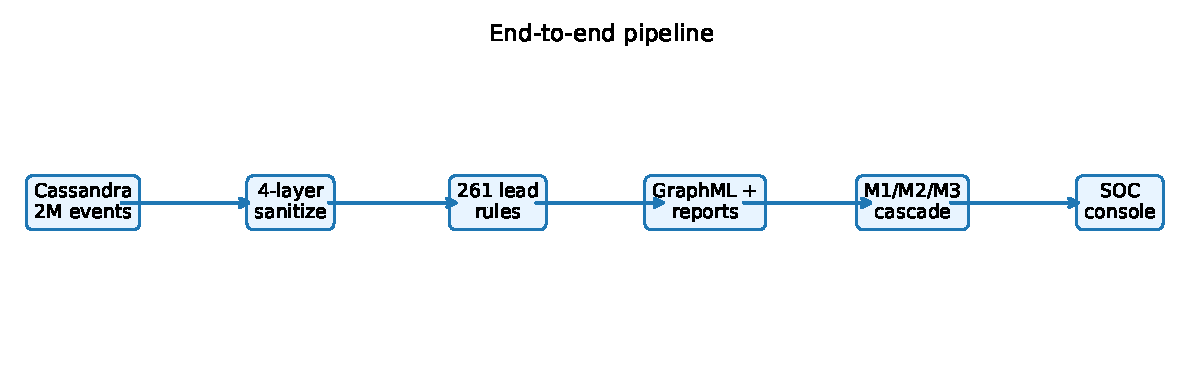
\includegraphics[width=0.95\linewidth]{figures/architecture.pdf}
\caption{Diagrama esquem\'atico end-to-end (requerido).}
\label{fig:arch}
\end{figure}

Evaluaremos con split temporal 80/20 (pasado entrena, futuro prueba), m\'etrica F1-macro + PR-AUC por
clase (nunca accuracy) y an\'alisis de complejidad por modelo. El despliegue previsto es FastAPI en
:8000 (\texttt{/score}, \texttt{/queue}, \texttt{/incident}) + consola React en el mismo origen
(Docker multi-stage), con bit\'acora de feedback para re-entrenar.

\section{Dataset: explicaci\'on y visualizaci\'on}

\texttt{witfoo/precinct6-cybersecurity} v2.1.0 (Apache-2.0): captura live 2024-07-26 $\to$ 08-01,
4 orgs, 19 productos / 12 vendors, 38 columnas por se\~nal, m\'as \texttt{incident\_signals}
hist\'orico (238,511), 47,585 nodos / 1,740,438 aristas y 51,371 incidentes con reporte.

\begin{table}[htbp]
\caption{Tiers live (IR $\approx$ 245:1).}
\label{tab:labels}
\centering
\begin{tabular}{@{}lrr@{}}
\toprule
Tier & Filas & \% \\
\midrule
benign & 1,897,153 & 94.31 \\
suspicious & 106,793 & 5.31 \\
malicious (1,584 incidentes) & 7,728 & 0.38 \\
\bottomrule
\end{tabular}
\end{table}

\begin{figure}[htbp]
\centering
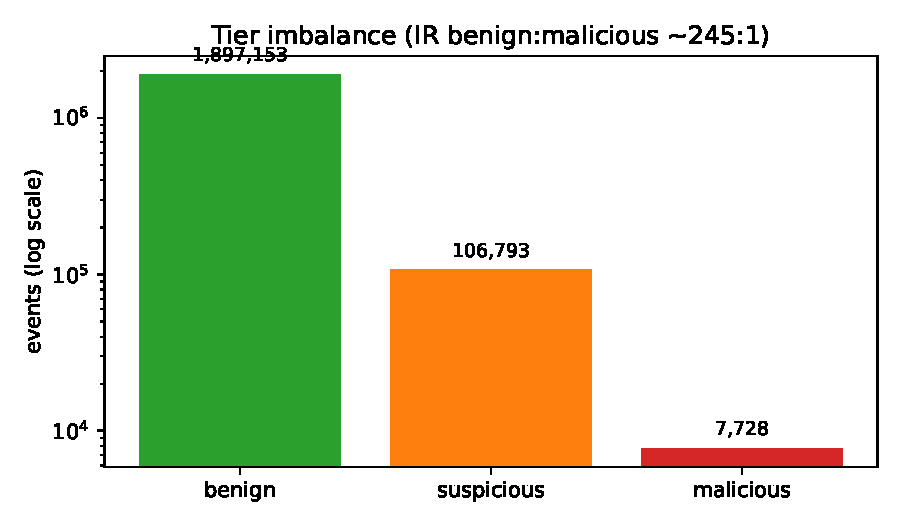
\includegraphics[width=0.48\linewidth]{figures/label_distribution.pdf}
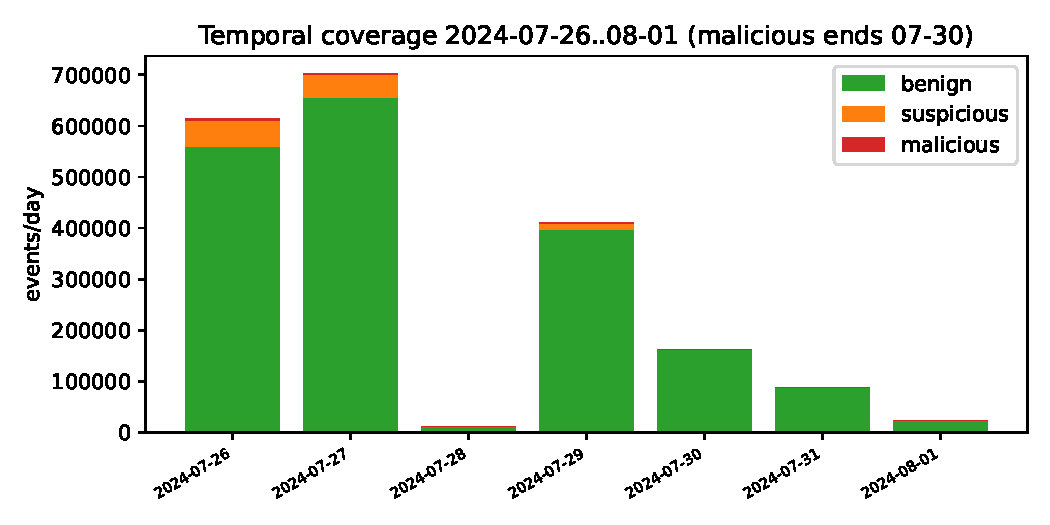
\includegraphics[width=0.48\linewidth]{figures/temporal_volume.pdf}
\caption{Exploraci\'on preliminar: desbalance (log) y cobertura temporal (malicious termina 07-30 $\to$ split temporal).}
\label{fig:data}
\end{figure}

La exploraci\'on preliminar (\texttt{src/eda\_report.py} $\to$ \texttt{reports/eda/}) muestra el
diccionario de 38 columnas, \texttt{severity} 49\% vac\'ia (= nivel propio, no mediana), priors ATT\&CK
que deber\'an excluirse de features (leakage), y tres hip\'otesis a verificar: tokens T1190 $\to$
componente de texto; vecinos $\pm$5\,min $\to$ componente de grafo; tier medio recuperable tabular.

\begin{thebibliography}{9}
\bibitem{devign} Y.~Zhou \emph{et al.}, ``Devign: effective vulnerability identification by learning comprehensive program semantics via graph neural networks,'' in \emph{NeurIPS}, 2019. arXiv:1909.03496.
\bibitem{cvssbert} M.~R.~Shahid y H.~Debar, ``CVSS-BERT: explainable NLP to determine the severity of a computer security vulnerability from its description,'' in \emph{IEEE ICMLA}, 2021. arXiv:2111.08510.
\bibitem{witfoo} WitFoo, Inc., ``Precinct6 cybersecurity dataset v2.1.0,'' HuggingFace, 2026.
\bibitem{attack} MITRE, ``ATT\&CK design and philosophy,'' 2020. \texttt{attack.mitre.org}.
\bibitem{nodlink} D.~Huang \emph{et al.}, ``NODLINK: online APT detection,'' in \emph{NDSS}, 2024. arXiv:2311.02331.
\bibitem{tram} MITRE CTID, ``Threat report ATT\&CK mapper (TRAM),'' \texttt{github.com/center-for-threat-informed-defense/tram}.
\bibitem{focal} T.-Y.~Lin \emph{et al.}, ``Focal loss for dense object detection,'' in \emph{ICCV}, 2017.
\bibitem{graphsage} W.~Hamilton \emph{et al.}, ``Inductive representation learning on large graphs,'' in \emph{NeurIPS}, 2017.
\bibitem{cyborg} M.~Stanton \emph{et al.}, ``CybORG: a gym for cyber operations,'' arXiv:2002.10667, 2020.
\end{thebibliography}

\end{document}
